% -*- latex -*-

\documentclass[twocolumn]{article}

\usepackage{amsfonts}
\usepackage{amssymb}
\usepackage{amsmath}
\usepackage{graphicx}
\usepackage{varioref}
\usepackage{fancyvrb}
\usepackage{cite}
\usepackage{subfigure}
\usepackage{xspace}
\usepackage[pdfstartview=FitH]{hyperref}

\title{Diverging Color Maps for Scientific Visualization}

\author{Kenneth~Moreland}

% Commands I use for citing.
\newcommand{\lcite}[1]{~\cite{#1}}
\newcommand{\scite}[1]{~\cite{#1}}

% Put figures inline with text when possible
\usepackage{float}
\floatplacement{figure}{htb}

% Avoid putting figures on their own page.
\renewcommand{\textfraction}{0.05}
\renewcommand{\topfraction}{0.95}

% Make sure this is big enough so that only big figures end up on their own
% page but small enough so that if a figure does have to be on its own
% page, it won't push everything to the bottom because it's not big enough
% to have its own page.
\renewcommand{\floatpagefraction}{.75}

\newcommand{\sticky}[1]{\textsc{[#1]}}

\newcommand{\RGB}{RGB\xspace}
\newcommand{\CMYK}{CMYK\xspace}
\newcommand{\XYZ}{XYZ\xspace}
\newcommand{\Lab}{CIELAB\xspace}
\newcommand{\Luv}{CIELUV\xspace}
\newcommand{\Msh}{Msh\xspace}
\newcommand{\DeltaE}{\ensuremath{\Delta{}E}\xspace}
\newcommand*{\cvec}[1]{\mathbf{#1}}

\begin{document}

\maketitle

\begin{abstract}
  One of the most fundamental features of scientific visualization is the
  process of mapping scalar values to colors.  This processes allows us to
  view scalar fields by coloring surfaces and volumes.  Dispite the
  importance of this mapping operation, the majority of scientific
  visualization tools and research are still using a color map that is
  famous for its ineffectiveness: the rainbow color map.  The rainbow color
  map, which na\"{i}vely sweeps through the most saturated colors a display
  can reproduce in the order of the colors in a rainbow, is well known for
  its abilities to obscure data, introduce artifacts, and confuse users.

  Although many other color maps have been proposed and used, none have
  been adopted by the visualization community as a good default in
  scientific visualization.  In this paper we explore the use of diverging
  color maps (sometimes also called bipolar color maps) for use in
  scientific visualization.  We conclude with a diverging color map that
  generally performs well in scientific visualization applications.  This
  color map is a clear replacement for the rainbow color map and can
  hopefully, once and for all, kill the use of the rainbow color map for
  serious scientific visualization applications.
\end{abstract}

\section{Introduction}
\label{sec:Introduction}

At its core, visualization is the process of providing a visual
representation of data.  One of the most fundamental and important aspects
of this process is the mapping of numbers to colors.  This mapping allows
us to pseudocolor an image or object based on varying numerical data.
Obviously, the choice of color map is important to allow the viewer to
easily perform the reverse mapping back to scalar values.

\begin{figure}
  \centering
  \includegraphics[width=2.5in]{images/RainbowBar}
  \caption{The rainbow color map.  Know thy enemy.}
  \label{fig:RainbowColorMap}
\end{figure}

By far the most common color map used in scientific visualization is the
rainbow color map, shown in Figure~\ref{fig:RainbowColorMap}.  In a recent
review on the use of color maps, Borland and Taylor\scite{Borland07} find
that the rainbow color map was used as the default in 8 out of the 9
toolkits they examined.  Borland and Taylor also find that in IEEE
Visualization papers from 2001 to 2005 the rainbow color map is used 51
percent of the time.

But despite its popularity, the rainbow color map has been shown to be a
poor choice for a color map in almost all problem domains.  This well
studied field of perception shows that the rainbow color map obfuscates,
rather than clarifies, the display of data in a variety of ways.  The
choice of a color map can be a complicated decision that changes based on
the visualization type and problem domain, but the rainbow color map is a
poor choice in almost all of them.

So why are so many visualization scientists and developers, experts who
should know better, still using the rainbow color map?  The answer is
unknown; there are many contributing factors.  Surely two main factors
heavily contribute.  The first is the ease at which the rainbow color map
can be created.  I myself am guilty of creating my first rainbow color map
long before learning anything about color spaces and human perception.  It
was my first choice and I was pleased with the colorful images, ignorant of
their dubious scientific value.

A second major contributor to the dominance of the rainbow color map is the
lack of a clear alternative, especially in terms of scientific
visualization.  There are certainly many publications that recommend some
very good choices for color maps\lcite{Ware04,Brewer05}.  However, each has
its sets of features and detractors, and the choice of the ``right'' one is
difficult.

This paper is a concluding report on the quest for finding a good default
color map for a general purpose scientific visualization application.  The
color map derived here is an all-around good performer: it works well for
low and high frequency data, orders the data, is perceptually linear,
behaves well for observers with color-deficient vision, and has reasonably
low impact on the shading of three dimensional surfaces.


\section{Previous Work}
\label{sec:PreviousWork}

This previous work section is divided into two parts.  The first part is a
quick review on previously proposed color maps and lists the benifits and
detractors of each.  The second section is a quick review on color spaces,
which are used heavily in the subsequent discussions in this paper.

\subsection{Color Maps}
\label{sec:PreviousWork:ColorMaps}

\begin{figure}
  \centering
  \includegraphics[width=2.5in]{images/GrayscaleBar}
  \caption{The grayscale color map.}
  \label{fig:GrayscaleColorMap}
\end{figure}
Let us start with perhaps the simplest color map of all: the grayscale
color map shown in Figure~\ref{fig:GrayscaleColorMap}.  Completely devoid
of any chromaticity, this map relies entirely on luminance to demonstrate
the numerical value.  Although a very simple map to create and use, this
map is surprisingly effective as the human visual system is most sensitive
to changes in luminance\lcite{Ware04,Mullen85}.  The grayscale color map is
used heavily in the image processing and medical visualization fields.

\begin{figure}
  \centering
  \begin{tabular}{c}
    \includegraphics[width=2.5in]{images/GrayscaleLocality} \\
    \includegraphics[width=2.5in]{images/BlackBodyLocality}
  \end{tabular}
  \caption{Pixels of the same luminance may look different depending on the
    surrounding pixels.}
  \label{fig:SimultaneousContrast}
\end{figure}
The grayscale color map also has a couple of detractors.  One problem is
that a human's perception to brightness is subject to the brightness of the
surrounding area.  Thus, when asked to compare the luminance of two objects
separated by distance and background, human subjects error up to 20\%.
This effect, is demonstrated in Figure~\ref{fig:SimultaneousContrast}, is
called simultaneous contrast\lcite{Stone05}.  Adding a chromaticity shift
helps, but does not fix the problem entirely.

Another problem with grayscale color maps that is of greater concern for
general purpose scientific visualization is its interference with surface
shading.  The shading of 3D surfaces based on light sources is of utmost
importance for perceiving the surface shape.  These shading cues are
composed almost entirely of luminance shifts.  Thus the luminance shift of
the grayscale color map mask the surface luminance shifts, especially in
the darker part of the spectrum as demonstrated in
Figure~\ref{fig:LuminanceVsShading}.  The problem cannot be corrected
without a major reduction in the range the luminance shifts in the color
map.

\begin{figure}
  \centering
  \includegraphics[width=1.25in]{images/GrayscaleShading}
  \includegraphics[width=1.25in]{images/IsoluminantShading}
  \caption{Maps with big changes in luminance hides shading cue important
    for determining 3D structure whereas isoluminant maps minimize shading
    interference.}
  \label{fig:LuminanceVsShading}
\end{figure}

\begin{figure}
  \centering
  \begin{tabular}{c}
    \includegraphics[width=2.5in]{images/Green2RedBar} \\
    \includegraphics[width=2.5in]{images/Cyan2MauveBar}
  \end{tabular}
  \caption{Isoluminant color maps.  The green to red color map is popular
    because it uses a pair of opponent colors, but the cyan to mauve color
    map is much easier to see by individuals with deuteranope or protanopic
    vision.}
  \label{fig:IsoluminantColorMap}
\end{figure}
Another class of color maps that is often suggested for use with 3D
surfaces is the isoluminant color map that is demonstrated in
Figure~\ref{fig:IsoluminantColorMap}.  Somewhat opposite to the grayscale
map, an isoluminant map maintains a constant (perceptual) luminance and
relies entirely on chromatic shifts.  An isoluminant color map is
theoretically ideal for mapping onto shaded surfaces, as is demonstrated in
Figure~\ref{fig:LuminanceVsShading}.

Isoluminant color maps are not without their detractors, however.  Human
perception is less sensitive to changes in saturation or hue than changes
in luminance, especially for high frequency data\lcite{Rogowitz96}.
Holding the luminance constant also restricts the colors that can be
represented.  Thus, the isoluminant color map will have a lower fidelity
than one in which the luminance is allowed to change.  Isoluminant color
maps also tend to look dull and ugly, which means that a casual user will
almost never choose one over a more vibrant color map like, say, the
rainbow color map.

However, as vibrant as the rainbow color map might be, it is actually an
extremely poor choice.  Based on the colors of light at different
wavelengths, the rainbow color map's design has nothing to do with how
humans perceive color.  This results in multiple problems when humans try
to do the reverse mapping from colors back to numbers.

The first problem with the rainbow color map is that it is sensitive to
deficiencies in vision.  A significant proportion of the population, most
of which are males, cannot distinguish between the red and green colors.
These unfortunate soles cannot distinguish many colors considered ``far
appart'' in the rainbow color map\lcite{Light04}.

The second problem is that the colors do not follow any natural perceived
ordering.  Perceptual experiments show that although a test subject, with
no prior training, will always order grayscale colors in order of luminance,
the test subjects will order rainbow colors in numerous different
ways\lcite{Ware04}.

\begin{figure}
  \centering
  \includegraphics[width=1.0in]{images/GrayscaleSpatialContrast}
  \qquad
  \includegraphics[width=1.0in]{images/RainbowSpatialContrast}
  \caption{A spatial contrast sensitivity function.  The frequency of the
    function increases from left to right, and the contrast increases from
    top to bottom.  Notice that the grayscale mapping faithfully reproduces
    the function.  The rainbow color mapping hides the variation in the low
    contrast region and appears less smooth in the high-contrast,
    low-frequency region.}
  \label{fig:RainbowSpatialContrast}
\end{figure}

A third problem is that the perceptual changes in the colors are not
uniform.  The colors appear to change faster in the cyan and yellow
regions, which can cause Mach bands in those regions.  The colors appear to
change slower in the blue, green, and red regions, which creates larger
bands of color.  Within these bands it can hide important changes in the
underlying data.  Thus, the nonuniform perceptual changes works to
simultaneously introduce artifacts and obfuscate real
data\lcite{Borland07} as demonstrated in
Figure~\ref{fig:RainbowSpatialContrast}.

These color maps comprise the most commonly used in literature and tools
today.  Other color maps are proposed by Ware\scite{Ware04} as well as
several others.  Most are similar in spirit to those here with uniform
changes in luminance, saturation, or hue or some combination thereof.

\subsection{Color Spaces}
\label{sec:PreviousWork:ColorSpaces}

The remainder of this paper relies on using different color spaces to
describe color map generation.  This section quickly reviews some of these
color spaces.

All color spaces are based on the tristimulus theory, which states that any
perceived color can be uniquely represented by a
3-tuple\lcite{Feynman63,Stone05} .  This result is a side effect of the
fact that there are exactly 3 different types of color receptors in the
human eye.

The color space most frequently used is the \RGB color space
\sticky{Reference}.  This color space is adopted by many graphics packages
such as OpenGL and is presented to users by just about every computer
application in existence that provides a color chooser.  The three values
in the \RGB color space refer to the intensity output by each of the three
wavelengths of light used by monitors, televisions, and projectors to
create colors.  There is also a similar \CMYK color space that defines
colors by how printers mix ink \sticky{Reference}.

Although the \RGB and \CMYK color spaces are good for many practical
purposes, they are defined exactly over the gamut of colors that can be
displayed, and it is sometimes useful to define colors over the gamut of
visible colors.  However, it is not as useful for describing colors that
are visible but not representable by the display.  To this end the
International Commission on Illumination (better known as CIE from its
French title, the \emph{Commission Internationale de l'\'{E}clairage})
convened in 1931 and defined the \XYZ color space \sticky{Reference}.  The
\XYZ color space provides a convenient way to consistently describe all
visible colors without being tied to any particular display device.

The \XYZ color space, however, is still defined by the physical properties
of light.  Movements within the \XYZ space are not perceptually linear.  To
address the need for a perceptually linear color space, the CIE developed
two more color spaces in 1976: \Lab and \Luv.  The choice between the two
is fairly arbitrary; this paper uses \Lab \sticky{Reference}.

\Lab is an approximation of how humans perceive light.  The Euclidean
distance between two points is the approximate perceived difference between
the two colors.  This Euclidean distance in \Lab space is known as \DeltaE
and makes a good metric for comparing color differences
\sticky{Reference?}.  This paper uses the notation
$\DeltaE\{\cvec{c_1},\cvec{c_2}\}$ to denote the \DeltaE for the pair of
colors $\cvec{c_1}$ and $\cvec{c_2}$.


\section{Color Map Requirements}
\label{sec:ColorMapRequirements}

Our ultimate goal is to design a color map that works well for in
general-purpose scientific visualization.  It should work well for a wide
breadth of tasks and users.  As such we have the following requirements.

\begin{itemize}
\item The map yields images that are aesthetically pleasing.
\item The map maximizes the perceptual resolution.
\item Interference the shading of 3D surfaces is minimal.
\item The map is not sensitive with vision deficiencies.
\item The order of the colors should be natural.
\item The perceptual interpolation matches the underlying scalars the map
  represents.
\end{itemize}

The reasoning behind most of these requirements is self explanatory.  The
requirement that the color map be ``pretty,'' however, is not one often
found in the scientific literature.  After all, the attractiveness of the
color map, which is difficult to quantify in the first place, has little to
do its effectiveness in conveying information.  Nevertheless, aesthetic
appeal is important as users will use that as a criteria in selecting
visualization products and generating images.

% \begin{itemize}
% \item Due to the proliferation of visualization programs and images using
%   the rainbow color map, many users will have ``learned'' the order of the
%   colors and will continue to have to use them.  Our color map should try
%   not to break that convention.
% \item Color maps often co-exist with other visible elements: labels,
%   backgrounds, auxiliary structures and features, annotation, etc.  Thus,
%   the color map should yield well other elements with carefully chosen
%   colors.
% \end{itemize}

Several of these requirements are contradictory, which makes choosing a
general purpose color map so difficult.  All of the examples in
Section~\ref{sec:PreviousWork:ColorMaps} excel in some of the requirements,
but fail completely in one or more of the others.  It is impossible to have
a color map that performs perfectly in all of the requirements.  Our color
map must be a compromise that works reasonable well in all areas.


\section{Color Map Design}
\label{sec:ColorMapDesign}

There are many color maps in existence today, but very few of them satisfy
all of the requirements listed in Section~\ref{sec:ColorMapRequirements}.
For inspiration, I look at the very mature field of cartography.  People
have been making maps for thousands of years.  Throughout the history of
cartography there has been much focus on both the effectiveness of
conveying information as well as the aesthetics of the design.

Brewer\scite{Brewer05} provides excellent advice for designing cartographic
color maps as well as many examples of well designed color
maps.\footnote{Brewer's color maps are also available on her web site:
  \href{http://www.colorbrewer.org}{www.colorbrewer.org}.} Brewer divides
her color maps into three classes: qualitative, sequential, and diverging.
Examples of these color maps are shown in Figure~\ref{fig:BrewerExamples}.

\begin{figure}
  \centering
  \subfigure[Qualitative]{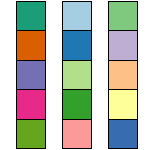
\includegraphics{images/ColorMapsQualitative}}
  \quad
  \subfigure[Sequential]{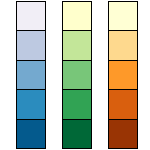
\includegraphics{images/ColorMapsSequential}}
  \quad
  \subfigure[Diverging]{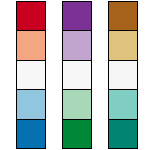
\includegraphics{images/ColorMapsDiverging}}
  \caption{Examples of color maps from
    \href{http://www.colorbrewer.org}{www.colorbrewer.org}.}
  \label{fig:BrewerExamples}
\end{figure}

The qualitative color maps are used to represent a collection of discrete,
unordered classes.  Since the colors have no ordering (by design), they are
not appropriate for mapping a scalar variable.

The sequential color maps are (nearly) monochromatic.  The range from a
heavily saturated color to various levels of unsaturation, terminating at
or close to white.  The monotonic nature of the saturation level maps well
to a scalar value.  Sequential maps are usually oriented such that the most
saturated color represents the lowest scalar value whereas the more
luminant white represents the highest scalar value.  However, the color
map, which has a limited range of luminance, can sometimes be flipped.  For
example, if a red or orange sequential color map represented temperature,
it would be more natural to represent the highest temperature with the most
saturated color.

The diverging color maps (also known as \sticky{look it up}) have two major
color components.  The map transitions from one color component to the
other by passing through an unsaturated color (white or yellow).  Diverging
color maps are typically used for to represent a scalar with a significant
value at or near the median.  For example, a color map for elevation could
put sea level at white with below sea level\lcite{Tufte97}.  The ordering
of the colors is usually based on the context with which they are used.  In
the elevation example, blues can be used to represent the sea floor depth
and tans can be used to represent land elevation.

Sequential color maps are clearly appropriate for scientific visualization.
Their monotonic nature yields well to mapping scalar values.  Diverging
color maps are a less obvious choice.  We cannot expect there to be some
significant median value that the diverging color map is designed to
highlight.

However, diverging color maps can better satisfy the requirements given in
Section~\ref{sec:ColorMapRequirements} then their sequential counterparts.
First, the more colorful nature of the diverging color map can be more
aesthetically pleasing.  Second, the diverget color map can have up to
twice the perceptual resolution of the sequential color map without
sacrificing the requirements of surface shading or accommodating viewers
with bi-chromatic \sticky{Correct?} vision.

What diverging color maps lack in general is a natural ordering of colors.
To impose a color ordering, we carefully chose two colors that most
naturally have ``low'' and ``high'' connotations.  We achieve this with the
concept of ``cool'' and ``warm'' colors \sticky{Cite}.  Color temperature
has been used for centuries as a means of evoking an emotional response.
The response is psychosomatic.  The resons for the interpretation are
unclear although it may have to do with how light at the opposite ends of
the visibile spectrum refract in the eye\lcite{Bailey06}.  We can best
evoke the cool-warm response by using blue and red for the low and high
extrema, respectively.

Using our initial criteria, we can think of diverging color map as
``locally'' optimal.  We cannot add any color to anywhere in the map
without degrading one or more of the requirements.


\subsection{Perceptual Uniformity}
\label{sec:PerceptualUniformity}

An important characteristic of any color map is that it is perceptually
uniform throughout.  For a discrete color map, perceptual uniformity means
that all pairs of adjacent colors will look equally different from each
other.  That is, the \DeltaE for each adjacent pair is (roughly) the same.

For a continuous color map, we want the rate of change for the color to be
constant.  If we characterize our color map with function $\cvec{c}(x)$
that takes scalar value $x$ and returns a color vector, the color map is
perceptually uniform if
\begin{equation}
  \lim_{\Delta{}x \rightarrow 0}{
    \frac{\DeltaE\{\cvec{c}(x),\cvec{c}(x+\Delta{x})}{\Delta{}x} }
  \label{eq:ContinuousDE}
\end{equation}
is constant for all valid $x$.

The easiest way to ensure that Equation~\ref{eq:ContinuousDE} is constant
is to linearly interpolate colors in the \Lab color space.  However, that
is not entirely possible to do for diverging color maps.  Lines from red to
blue will not go through white.  A piecewise linear interpolation is mostly
effective, but can create an artificial Mach band at white where the
luminance sharply transitions from increasing to decreasing as demonstrated
in Figure~\ref{fig:LinearMachBands}.

\begin{figure}
  \centering
  \includegraphics[width=1in]{images/Cool2WarmLabRadial}
  \qquad
  \includegraphics[width=1in]{images/Cool2WarmRadial}
  \caption{Using piecewise linear interpolations in \Lab color space causes
    Mach bands in the white part of diverging color maps (left image).  The
    problem can be corrected by interpolating in \Msh space (right image).}
  \label{fig:LinearMachBands}
\end{figure}

Rather than have a sharp transition in the luminance, we require a
``leveling off'' of the luminance as the color map approaches white.  To
compensate, the chromaticity must change more dramatically in this part of
the color map.  A method for designing this type of color map is defined in
the next section.

\subsection{\Msh Color Space}
\label{sec:MshColorSpace}

To simplify the design of continuous, diverging color maps, I derive a new
color space called \Msh.  \Msh is basically a polar form of the \Lab color
space.  $M$ is the magnitude of the vector, $s$ (the saturation) is the
angle away from the $L*$ axis, and $h$ (the hue) is the angle of the
vector's projection in the $a*$-$b*$ plane.  Conversion between the two
color spaces is straightforward.

\begin{equation}
  \begin{split}
    M &= \sqrt{{L*}^2 + a*^2 + b*^2} \\
    s &= \arccos\left(\frac{L*}{M}\right) \\
    h &= \arctan\left(\frac{b*}{a*}\right)
  \end{split}
  \label{eqn:LabToMsh}
\end{equation}

\begin{equation}
  \begin{split}
    L* &= M \cos\left(s\right) \\
    a* &= M \sin\left(s\right) \cos\left(h\right) \\
    b* &= M \sin\left(s\right) \sin\left(h\right)
  \end{split}
\end{equation}

Note that \Msh, like all polar coordinates, has a pole in which one of the
coordinates is ill defined.  Specifically, when $s = 0$ (the color is on
the $L$ axis), $h$ has no effect.  This pole was chosen because it
coincides with a singularity in human vision.  When saturation is low, the
color has no hue.  It is therefor possible to make a discontinuous jump
in the hue while still maintaining perceptual continuance.

Piecewise linear interpolations in \Msh space behave very well for
diverging color maps.  As $s$ linearly approaches zero, the luminance
naturally levels out while the chromaticity changes faster.  Although this
will lead to a more significant rate of change in the chromaticity, it will
not be noticeable as it coincides with a singularity in perception.  In
fact, we can make a jump in the value of the hue at that point without it
being noticeable.

An ideal way to build a diverging color map in \Msh space is to start at
one color, linearly reduce $s$ to 0 (to get white), flip $h$ to the
appropriate value for the last color, and then linearly increase $s$ to the
desired value.  Unfortunately, this strategy tends to produce colors that
are not reproducible by physical display systems.  We can correct for this
problem by reducing $M$ at each end, but this adds the problem that colors
will change faster near white when $M$ is larger.

We can restore the uniformity of the color map again by adding some
``spin'' to the hue.  Even though $h$ is interpolated linearly, the changes
have a greater effect on the color when $s$ is larger, which can
counterbalance the growing $M$.  The next section describes how to chose an
appropriate hue change.

\subsection{Choosing a Hue Spin}
\label{sec:ChoosingAHueSpin}

Let us consider the transition from a saturated color, $\cvec{c}_s=(M_s,
s_s, h_s)$, at an end of the color map to an unsaturated ``white'' color,
$\cvec{c}_u=(M_u, 0, h_u)$, at the beginning of the color map.  As the
color map moves from $\cvec{c}_s$ to $\cvec{c}_u$, the $M$, $s$, and $h$
coordinates are varied linearly.  The slope of these coordinates can be
characterized as $M_m = M_u - M_s$, $s_m = -s_s$, and $h_m = h_u - h_m$.
(Note that $h_u$ has no effect on the unsaturated color, but is provided to
conveniently define the rate of change.)

\begin{figure}
  \centering
  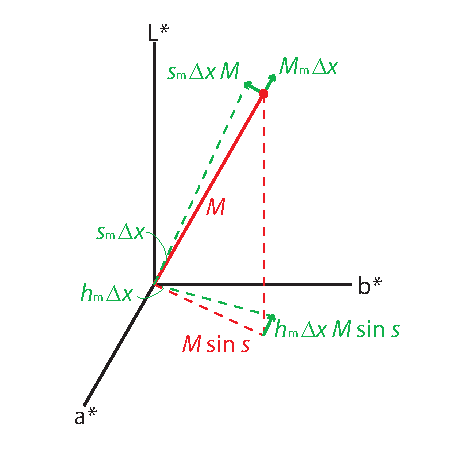
\includegraphics[height=1.5in]{images/MshDeltaMovements}
  \caption{A small linear movement in \Msh space}
  \label{sec:LinearMshMovement}
\end{figure}

Figure~\ref{sec:LinearMshMovement} shows how a small movement in this
linear \Msh function behaves in \Lab space.  The distance measurements take
advantage of the property that if you rotate a vector of radius $r$ by some
small angle $\Delta\alpha$, then the change in the vector is
$\lim_{\Delta\alpha \rightarrow 0}r \Delta\alpha$.  Clearly the \DeltaE,
the magnitude of change in \Lab space, is
\begin{equation}
  \sqrt{(M_m \Delta x)^2 + (s_m \Delta x M)^2 + (h_m \Delta x M \sin s)^2}
  \label{eq:DeltaEforLinearMshMovement}
\end{equation}

Equation~\ref{eq:DeltaEforLinearMshMovement} will not be constant unless
$M$ and $h_m$ is zero which, as described in the previous section, is
unacceptable.  However we can get pretty close to constant by choosing
$h_u$ so that Equation~\ref{eq:DeltaEforLinearMshMovement} is equal for
$\cvec{c}_s$ and $\cvec{c}_u$.

\begin{multline*}
  \sqrt{(M_m \Delta x)^2 + (s_m \Delta x M_s)^2 + (h_m \Delta x M_s \sin s_s)^2}
  \\ =
  \sqrt{(M_m \Delta x)^2 + (s_m \Delta x M_u)^2}
\end{multline*}

Note that the right side of the equation is missing a term because it
evaluates to 0 for the unsaturated color.  We can safely get rid of the
square roots because there is a sum of square real numbers inside them
both.

\begin{align}
    (M_m \Delta x)^2 + (s_m M_s)^2 \quad & \notag \\
    + (h_m M_s \sin s_s)^2 &= (M_m \Delta x)^2 + (s_m M_u)^2 \notag \\
    h_m^2 M_s^2 \sin^2 s_s &= s_m^2 (M_u^2 - M_s^2) \notag \\
    h_m^2 &= \frac{s_m^2 (M_u^2 - M_s^2)}{M_s^2 \sin^2 s_s} \notag \\
    h_m &= \pm \frac{s_m \sqrt{M_u^2 - M_s^2}}{M_s \sin s_s}
    \label{eqn:adjusted_hm}
\end{align}

Remember that $s_m=-s_s$.  We can use Equation~\ref{eqn:adjusted_hm} to
determine a good hue to use for the white point (from the given side).

\begin{equation}
  h_u = h_s \pm \frac{s_s \sqrt{M_u^2 - M_s^2}}{M_s \sin s_s}
  \label{eqn:adjusted_hu}
\end{equation}

Note that Equation~\ref{eqn:adjusted_hu} will most certainly yield a
different value for each of the saturated colors used in the diverging
color map.  The direction in which the hue is ``spun'' is unimportant with
regard to perception.  I usually adjust the hue to be away from 0 because
it provides slightly more aesthetically pleasing results.


\section{Results}
\label{sec:Results}

\begin{figure}
  \centering
  \includegraphics[width=2.5in]{images/Cool2WarmBar}
  \caption{A continuous diverging color map well suited to scientific
    visualization.}
  \label{fig:Cool2WarmBar}
\end{figure}

Applying the design described in Section~\ref{sec:ColorMapDesign} results
in the color map shown in Figure~\ref{fig:Cool2WarmBar}.  The control
points, to be interpolated in \Msh space, are given in
Table~\ref{table:Cool2Warm}.  \sticky{It would be nice to provide a large
  table containing the full range of colors.  How can I best do that?  A
  web link?  Where?}

\begin{table}
  \centering
  \caption{Cool to warm color map control points.}
  \begin{tabular}{c@{\qquad}ccc}
    Color & M & s & h \\
    \hline
    Red & 77 & 0.95 & 0.5 \\
    White & 95 & 0 & 1.34/-2.35 \\
    Blue & 70 & 0.9 & -1.3
  \end{tabular}
  \label{table:Cool2Warm}
\end{table}

This diverging color map works admirably for all of our scientific
visualization requirements.  The colors are asthetically pleasing, the
order of the colors is natural, the rate of change is perceptually linear,
and the colors are still easily distinguished by those with bichromatic
\sticky{Correct?} vision.  The map also has a good perceptual range and
minimally interfears with shading, as demonstrated in
Figure~\ref{fig:Cool2WarmResponse}.

\begin{figure}
  \centering
  \includegraphics[height=1in]{images/Cool2WarmSpatialContrast}
  \quad
  \includegraphics[height=1in]{images/Cool2WarmShading}
  \caption{The spatial contrast response (left) and effect on shading
    (right) of the diverging color map.}
  \label{fig:Cool2WarmResponse}
\end{figure}

In addition, dispite having a relatively large perceptual response, the
color map still allows for a significant amount of annotation added as
shown in Figure~\ref{fig:ColorMapWithAnnotation}.

\begin{figure}
  \centering
  \includegraphics[width=3in]{images/AnnotationExample}
  \caption{Terrain with the color map applied and heavily annotated. \sticky{An example invovling sci vis would probably be better.  Do we have anything?}
  \label{fig:ColorMapWithAnnotation}
\end{figure}

Using the techniques described in Section~\ref{sec:ColorMapDesign}, we can
also design continuous diverging color maps with different colors.  Such
color maps may be useful in domain specific situations when colors have
specific meaning.  Some examples are given in
Figure~\ref{fig:OtherColorMaps}.

\begin{figure}
  \centering
  \sticky{More diverging color maps.}
  \caption{Further examples of color maps.}
  \label{fig:OtherColorMaps}
\end{figure}

\sticky{Is there anything else I can put in the results section?  Is there
  some less qualitative evidence that this is a good color map?}


\section{Discussion}
\label{sec:Discussion}

This paper provides a color map that is a good all-around performer for
scientific visualization.  The map is an effective way to communicate data
through colors.  Because its endpoints match those of the horrible rainbow
color map most often currently used, it can be used as a drop-in
replacement.

Although we have not been able to do user studies, the design of this color
map is based on well established theories on color perception.  This map is
a clear improvement over what is commonly used today, and I hope that many
will follow in adopting it as the new standard.


\section{Acknowledgements}

This work was done at Sandia National Laboratories.  Sandia is a
multiprogram laboratory operated by Sandia Corporation, a Lockheed Martin
Company, for the United States Department of Energy's National Nuclear
Security Administration under contract DE-AC04-94AL85000.

\bibliographystyle{plain}
\bibliography{ColorMaps}

\end{document}
